\documentclass[handout]{beamer}

\usepackage{fontspec} 
% \usepackage{lsp-makros}
\useoutertheme{lsp}

\usepackage{lsptitle}

\def\two@digits#1{\ifnum#1<10 0\fi\number#1}
\def\mytoday{\two@digits{\number\day}.\two@digits{\number\month}.\number\year}


\usepackage{xspace,multicol}
\newcommand{\latex}{\LaTeX\xspace}
\usepackage{tikz}


\newcounter{lastpagemainpart}
\footnotesep0pt
\renewcommand{\footnoterule}{}
\usefootnotetemplate{
  \noindent
  \insertfootnotemark\insertfootnotetext}

\let\beamerfn=\footnote
\renewcommand{\footnote}[1]{%
\let\oldfnsize=\footnotesize%
\let\footnotesize=\tiny%
\beamerfn<\thebeamerpauses->{#1}%
\let\footnotesize=\oldfnsize}


\date{\mbox{2018-09-04, HIRMEOS Workshop, SUB Göttingen}}
% \newline HIRMEOS Workshop: Entity-Fishing for Digital Humanities and Scholarly Publishing, SLUB Göttingen}

\usepackage{eurosym}  
 
\renewcommand{\centerline}[1]{\hfill#1\hfill\hfill\mbox{}}


\title{Retrieving entities from publications in linguistics}%: Glottolog and Concepticon}
\institute{Language Science Press}
\author[LangSci]{Sebastian Nordhoff}



\begin{document}
\lspbeamertitle
\section{linguistics}
\frame{
\frametitle{linguistics}
\begin{itemize}
 \item  monograph
 \item  longer
 \item  less output than biology for instance
 \item  less digging
 \item  Umfrage
\end{itemize}
}
       
       
\frame{
\frametitle{How do linguists search for literature}
  \begin{itemize} 
  \item  Umfrage
  \end{itemize}
}
       
       
       
       
\section{LangSci}
\frame{
  \frametitle{Language Science Press}
  \begin{itemize}
  \item  75 books; 22 series  
  \end{itemize}
  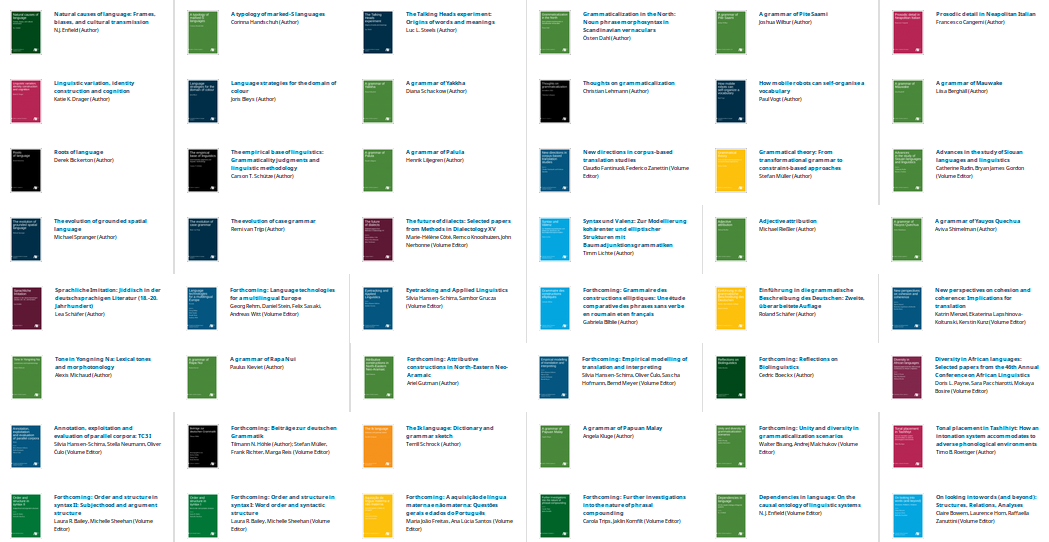
\includegraphics[height=\textheight]{catalog.png}
}

\frame{
\frametitle{}
\begin{itemize}
 \item         formats
 \begin{itemize}
  \item pdf
  \item tex
  \item bib
 \end{itemize}             
 \item Indexes 
 \begin{itemize}
  \item Language index
  \item Subject index 
  \item Name index
 \end{itemize} 
\end{itemize}
}
 

\frame{
\frametitle{\raggedright Bootstrapping index with sketchengine}
\begin{tabularx}{\textwidth}{XX}
image composition  \newline                
eye tracking       \newline           
speaking direction         \newline         
typographic identity     \newline             
fixation duration        \newline          
audiovisual translation  \newline                
aesthetic experience     \newline             
title area               \newline   
film material            \newline      
speaker identification   \newline               
film title               \newline   
natural focus            \newline      
text element             \newline     
image track              \newline    
information intake       \newline
graphical translation     \newline            
&
title placement           \newline      
bottom-centre area        \newline         
typographic film          \newline       
german image              \newline   
split attention           \newline      
gaze behaviour            \newline     
reading speed             \newline    
film identity             \newline    
typographic film identity \newline                
tracking research         \newline        
first fixation            \newline     
additional language       \newline          
narrative text            \newline     
eye tracking research     \newline            
visual attention          \newline       
individual placement      \newline   
\end{tabularx}
}

             
\section{NERD}
\frame{
\frametitle{NERD} 

\includegraphics[height=.4\textheight]{hirmeoslogo.jpg}
}

\frame{
\frametitle{Goals}
\begin{itemize}
 \item         higher goals
 \begin{itemize}
  \item exploration: \\
  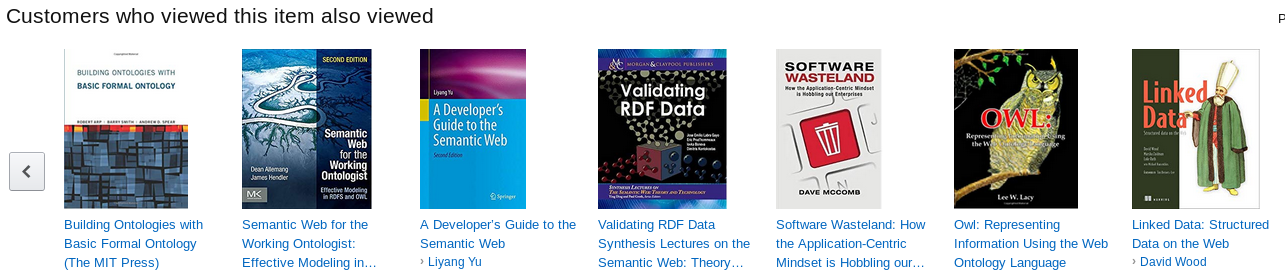
\includegraphics[height=2cm]{alsoviewed.png}
  \item automated reasoning
  \begin{itemize}
   \item gene $\longleftrightarrow$ ~protein 
   \item ~\hphantom{gene $\longleftrightarrow$ }protein $\longleftrightarrow$ disease
   \item gene $\longleftrightarrow$ ~protein $\longleftrightarrow$ disease
  \end{itemize}
 \end{itemize}          
\end{itemize}
}
\frame{
\frametitle{Goals}
\begin{itemize} 
 \item  stated goals
 \begin{itemize}
  \item   enhance discoverability
  \item   aggregation (word clouds)
  \item   generate collections 
  \item   highlighting
 \end{itemize}           
\end{itemize}
}

\frame{
\frametitle{}
\begin{itemize}
 \item         relevant knowledge bases
            authority
                gnd
                Orcid
            languoids
                glottolog
            concepts
                GOLD
                concepticon
\end{itemize}
}

\frame{
\frametitle{ linking entities}
\begin{itemize}
 \item keywords
 \item  person names
 \item language names
 \item concepts
\end{itemize}
}

\frame{
\frametitle{}
\begin{itemize}
 \item       keywords
                mixtec
\end{itemize}
}

\frame{
\frametitle{}
\begin{itemize}
 \item             person names
                saussure
                A. Lee
\end{itemize}
}

\frame{
\frametitle{}
\begin{itemize}
 \item             language names
                komnzo
\end{itemize}
}

\frame{
\frametitle{}
\begin{itemize}
 \item             concepts
                cross-linguistic categories don't exist
                GOLD
                    inallative 
                    romani ite domum
\end{itemize}
}

       
      



\section{Test}
\frame{
\frametitle{test}
: Hölzl, Andreas. 2018.  "A typology of questions in North-East asia and beyond"
}


\frame{
\frametitle{mongolic}
\begin{itemize}
 \item 
\end{itemize}
}

\frame{
\frametitle{Questions and conclusions}
\begin{itemize}
 \item 
\end{itemize}
}

 
%\setcounter{framenumber}{\thelastpagemainpart}
\end{document}